\documentclass[12pt]{article}
\usepackage[margin=1in]{geometry}
\usepackage{graphicx}
\usepackage{booktabs}
\usepackage{float}
\usepackage{caption}
\usepackage{hyperref}
\usepackage{enumitem}
\usepackage{titlesec}
\usepackage{lmodern}
\renewcommand{\familydefault}{\sfdefault}

\titleformat{\section}{\large\bfseries}{\thesection}{1em}{}
\titleformat{\subsection}{\normalsize\bfseries}{\thesubsection}{1em}{}

\title{Student Performance Visualization and Reporting}
\author{DataNinjas}
\date{\today}

\begin{document}

\maketitle


\section{Objective}
The project aims to create a Python-based visualization dashboard and detailed report that analyzes student performance across various demographic and educational factors. The final report highlights key trends, statistical summaries, and performance disparities in a professional, easy-to-understand format.

\section{Data Source}
\begin{itemize}[leftmargin=1.5em]
    \item \textbf{Dataset:} \texttt{StudentsPerformance.csv}
    \item \textbf{Format:} CSV
    \item \textbf{Total Records:} 1,000 students
\end{itemize}

\section{Summary Statistics}
\begin{itemize}[leftmargin=1.5em]
    \item \textbf{Total Number of Students:} 1000
    \item \textbf{Number of Male and Female Students:}
    \begin{itemize}
        \item Male: 482 (48.2\%)
        \item Female: 518 (51.8\%)
    \end{itemize}
    \item \textbf{Number of Students per Race/Ethnicity Group:}
    \begin{itemize}
        \item Group A: 89 (8.9\%)
        \item Group B: 190 (19.0\%)
        \item Group C: 319 (31.9\%)
        \item Group D: 262 (26.2\%)
        \item Group E: 140 (14.0\%)
    \end{itemize}
    \item \textbf{Number of Students by Test Preparation Status:}
    \begin{itemize}
        \item Completed: 358
        \item None: 642
    \end{itemize}
    \item \textbf{Number of Students by Lunch Type:}
    \begin{itemize}
        \item Standard: 645
        \item Free/Reduced: 355
    \end{itemize}
    \item \textbf{Average, Minimum, Maximum Scores per Subject:}
\end{itemize}

\begin{table}[H]
\centering
\caption{Score Summary Statistics}
\begin{tabular}{lccc}
\toprule
\textbf{Subject} & \textbf{Average} & \textbf{Minimum} & \textbf{Maximum} \\
\midrule
Math    & 66.09 & 0.00 & 100.00 \\
Reading & 69.17 & 17.00 & 100.00 \\
Writing & 68.05 & 10.00 & 100.00 \\
\bottomrule
\end{tabular}
\end{table}

\section{Charts Used and Rationale}

\begin{table}[H]
\centering
\caption{Charts Used and Their Purpose}
\begin{tabular}{p{4cm} p{5cm} p{5cm}}
\toprule
\textbf{Chart} & \textbf{What It Shows} & \textbf{Why It Was Used} \\
\midrule
Box Plot: Scores by Gender & Distribution and variability of math, reading, and writing scores for male and female students & To identify performance gaps and score spread between genders \\
Box Plot: Scores by Test Preparation Course & Score distributions for students who completed or did not complete test preparation & To assess the effectiveness of test preparation courses \\
Bar Chart: Avg Scores by Parental Education & Average subject scores by parental education level & To reveal correlation between parental education and student success \\
Bar Chart: Avg Scores by Lunch Type & Average subject scores by lunch type (standard vs. free/reduced) & To highlight disparities based on lunch type as a proxy for socioeconomic status \\
Bar Chart: Avg Scores by Race/Ethnicity & Average subject scores by race/ethnicity group & To understand demographic performance variations \\
Histogram: Score Distributions & Distribution and concentration of scores for each subject & To detect skewness and outliers in subject scores \\
Correlation Heatmap: Subject Scores & Correlation coefficients between math, reading, and writing scores & To understand cross-subject performance trends \\
Grouped Bar Chart: Test Preparation Impact by Gender & Test preparation effect on scores, segmented by gender & To assess gender-specific impact of test preparation \\
\bottomrule
\end{tabular}
\end{table}

\section{Visualizations and Key Insights}

\subsection{Box Plot: Scores by Gender}
\begin{figure}[H]
    \centering
    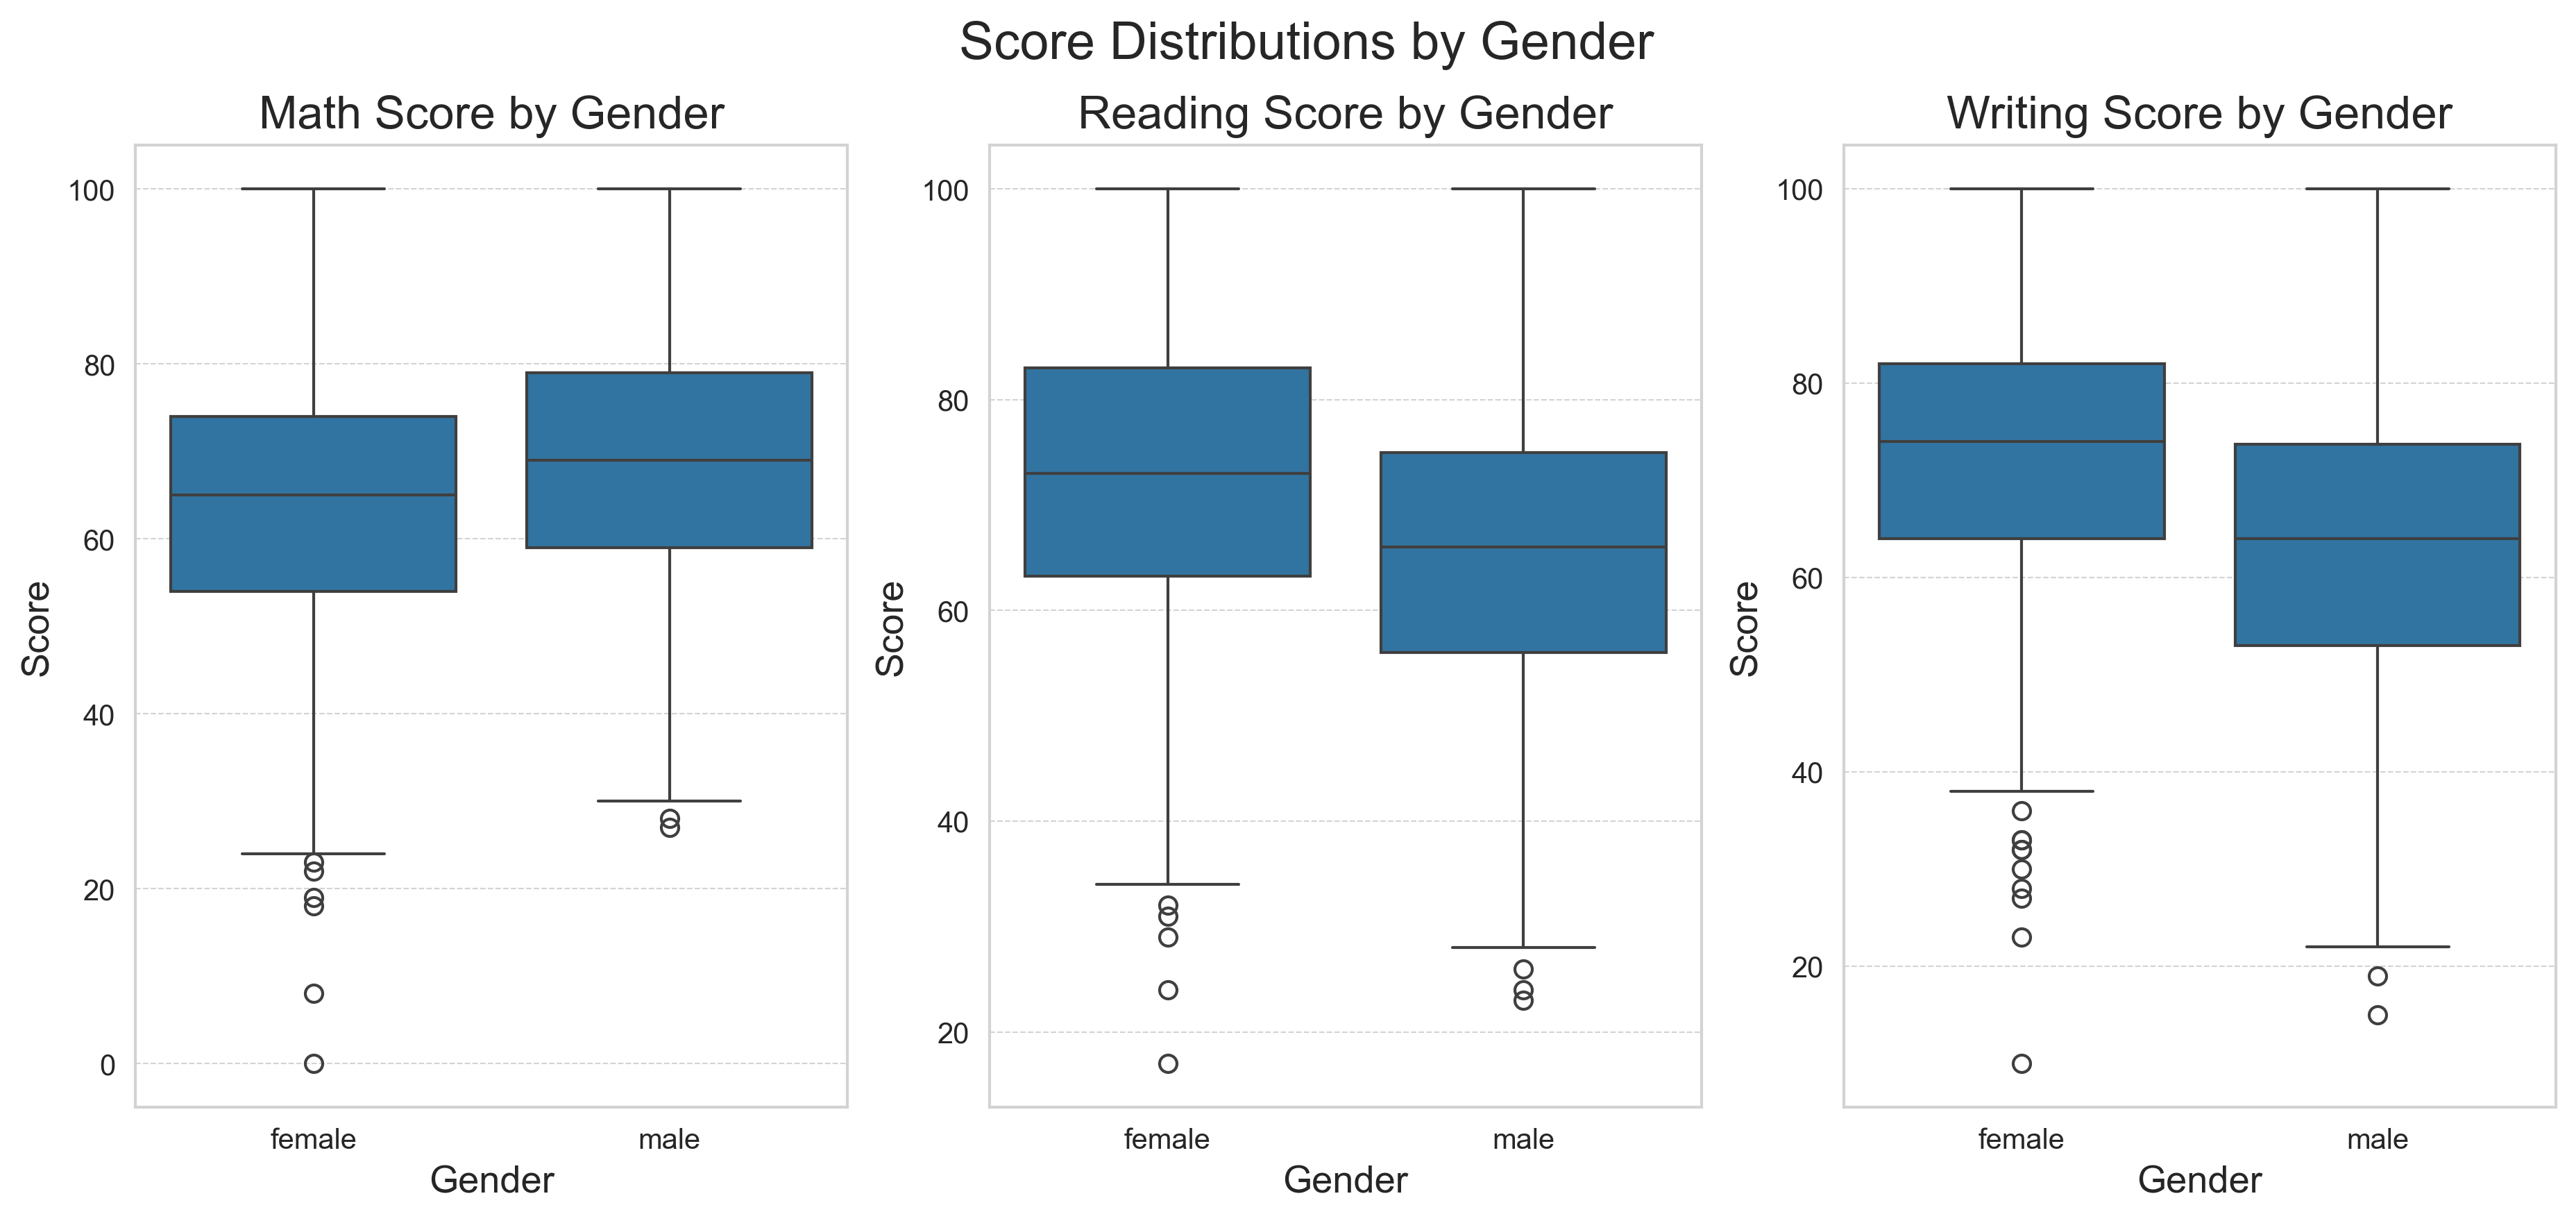
\includegraphics[width=0.8\textwidth]{figures/boxplot_scores_by_gender.png}
    \caption{Distribution of Math, Reading, and Writing Scores by Gender}
\end{figure}
\textbf{Key Insight:} Female students outperform males in reading and writing, while males have higher average math scores. Score distributions show greater variability among males in math.

\subsection{Box Plot: Scores by Test Preparation Course}
\begin{figure}[H]
    \centering
    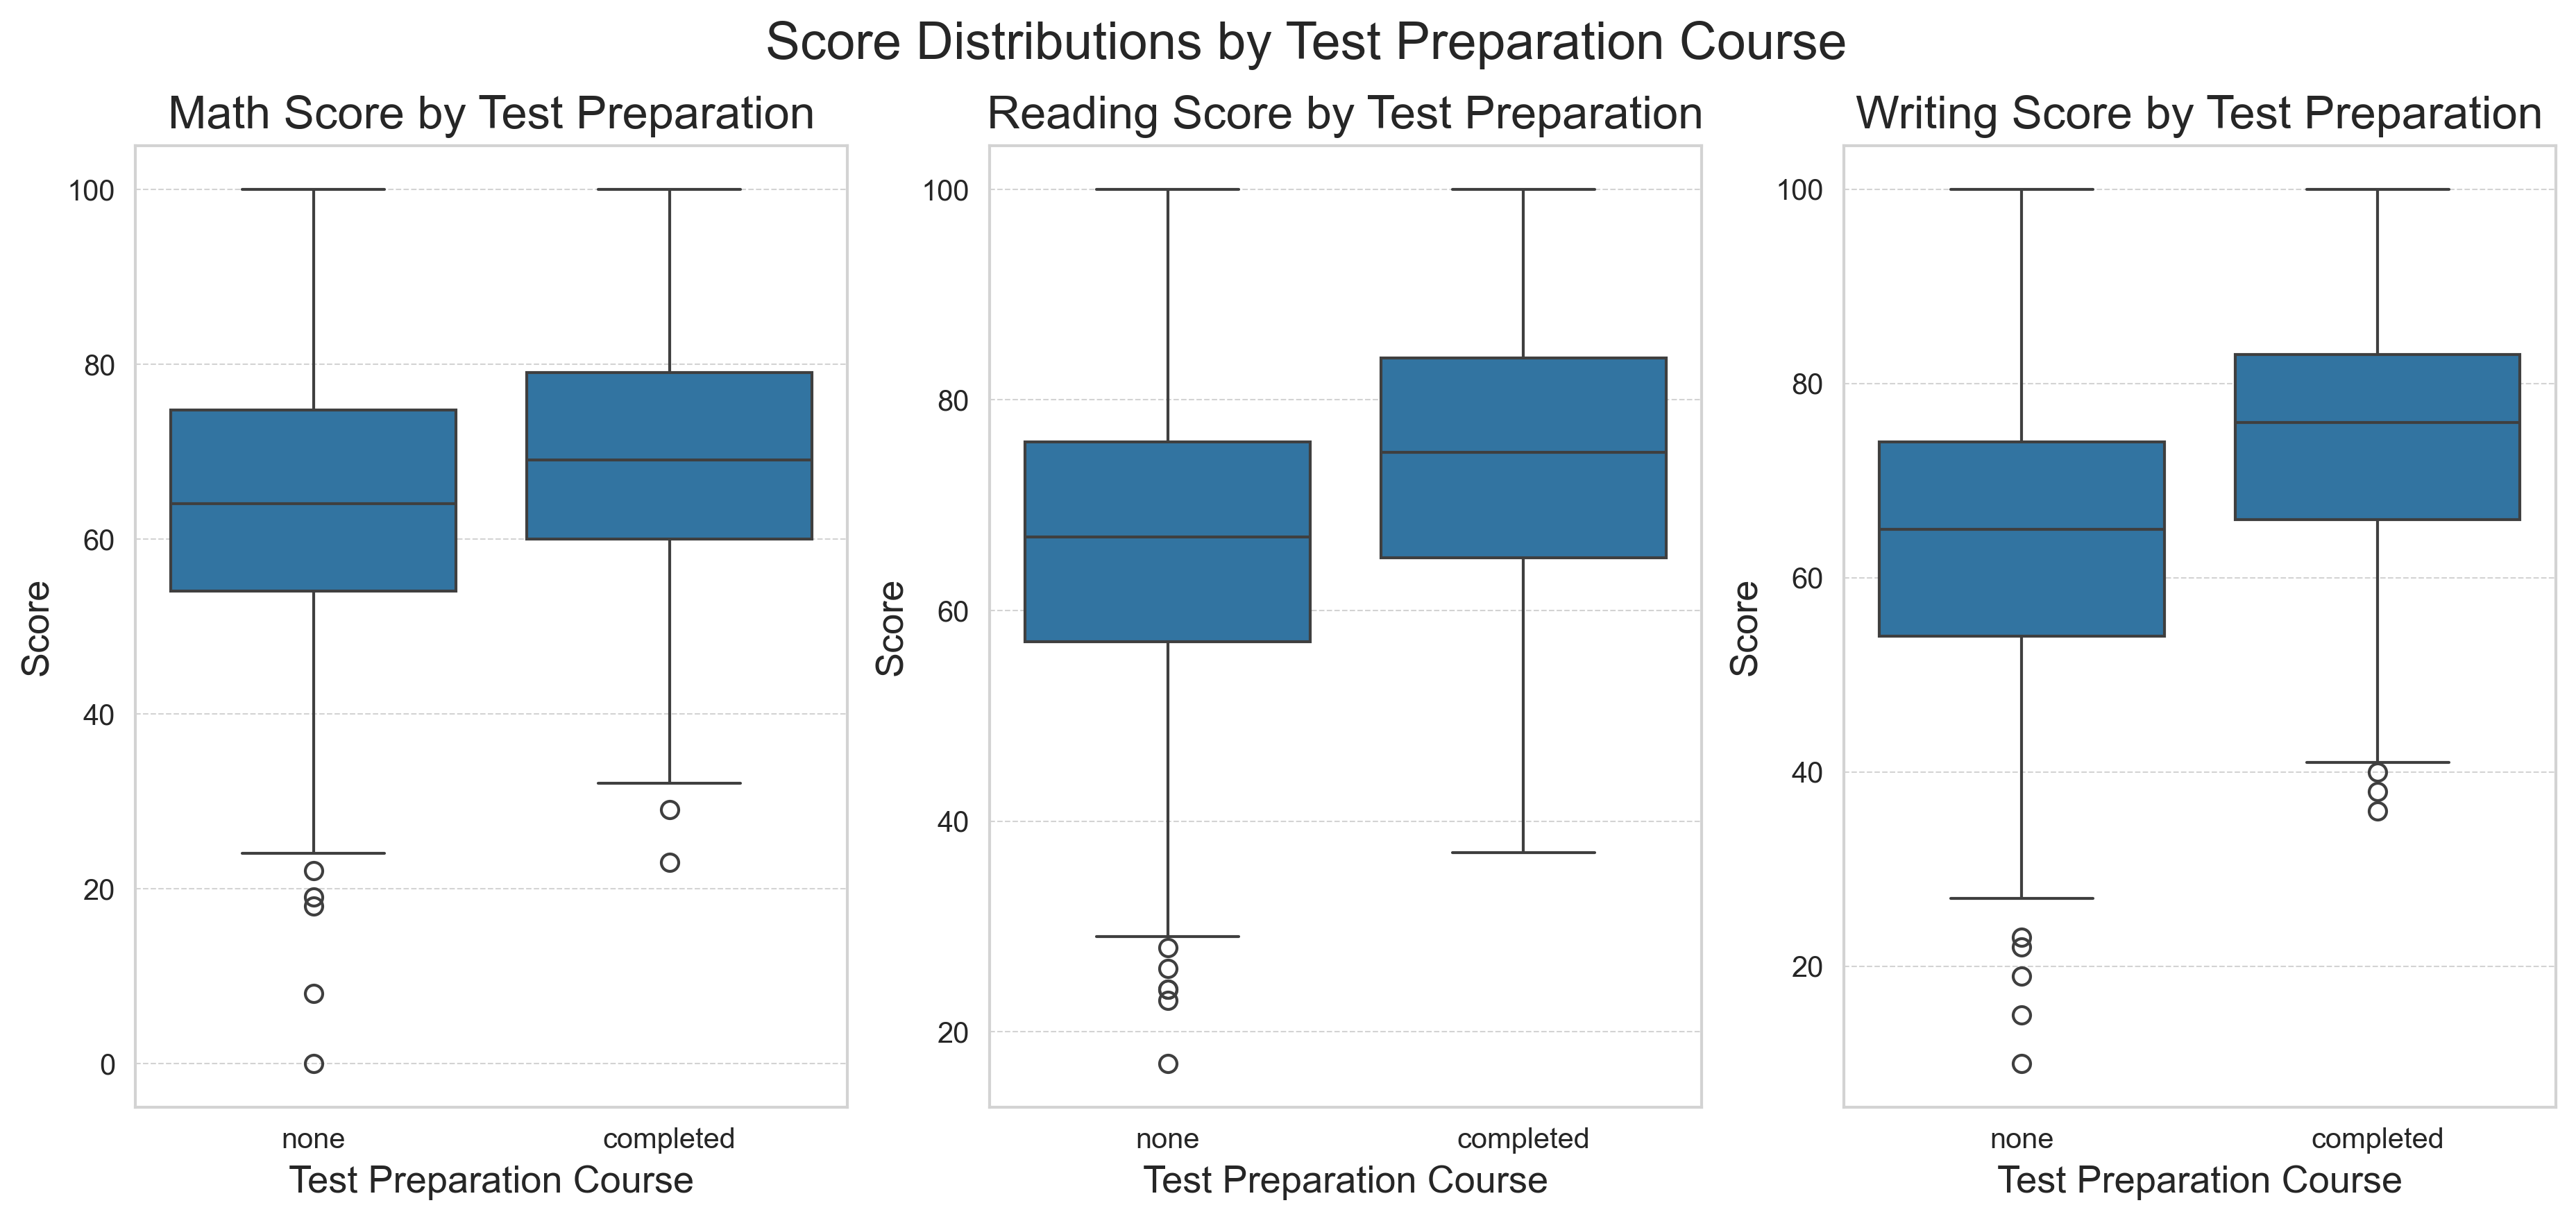
\includegraphics[width=0.8\textwidth]{figures/boxplot_scores_by_testprep.png}
    \caption{Distribution of Scores by Test Preparation Course}
\end{figure}
\textbf{Key Insight:} Students who completed the test preparation course scored higher on average in all subjects, with the most pronounced effect in writing and reading.

\subsection{Bar Chart: Average Scores by Parental Education}
\begin{figure}[H]
    \centering
    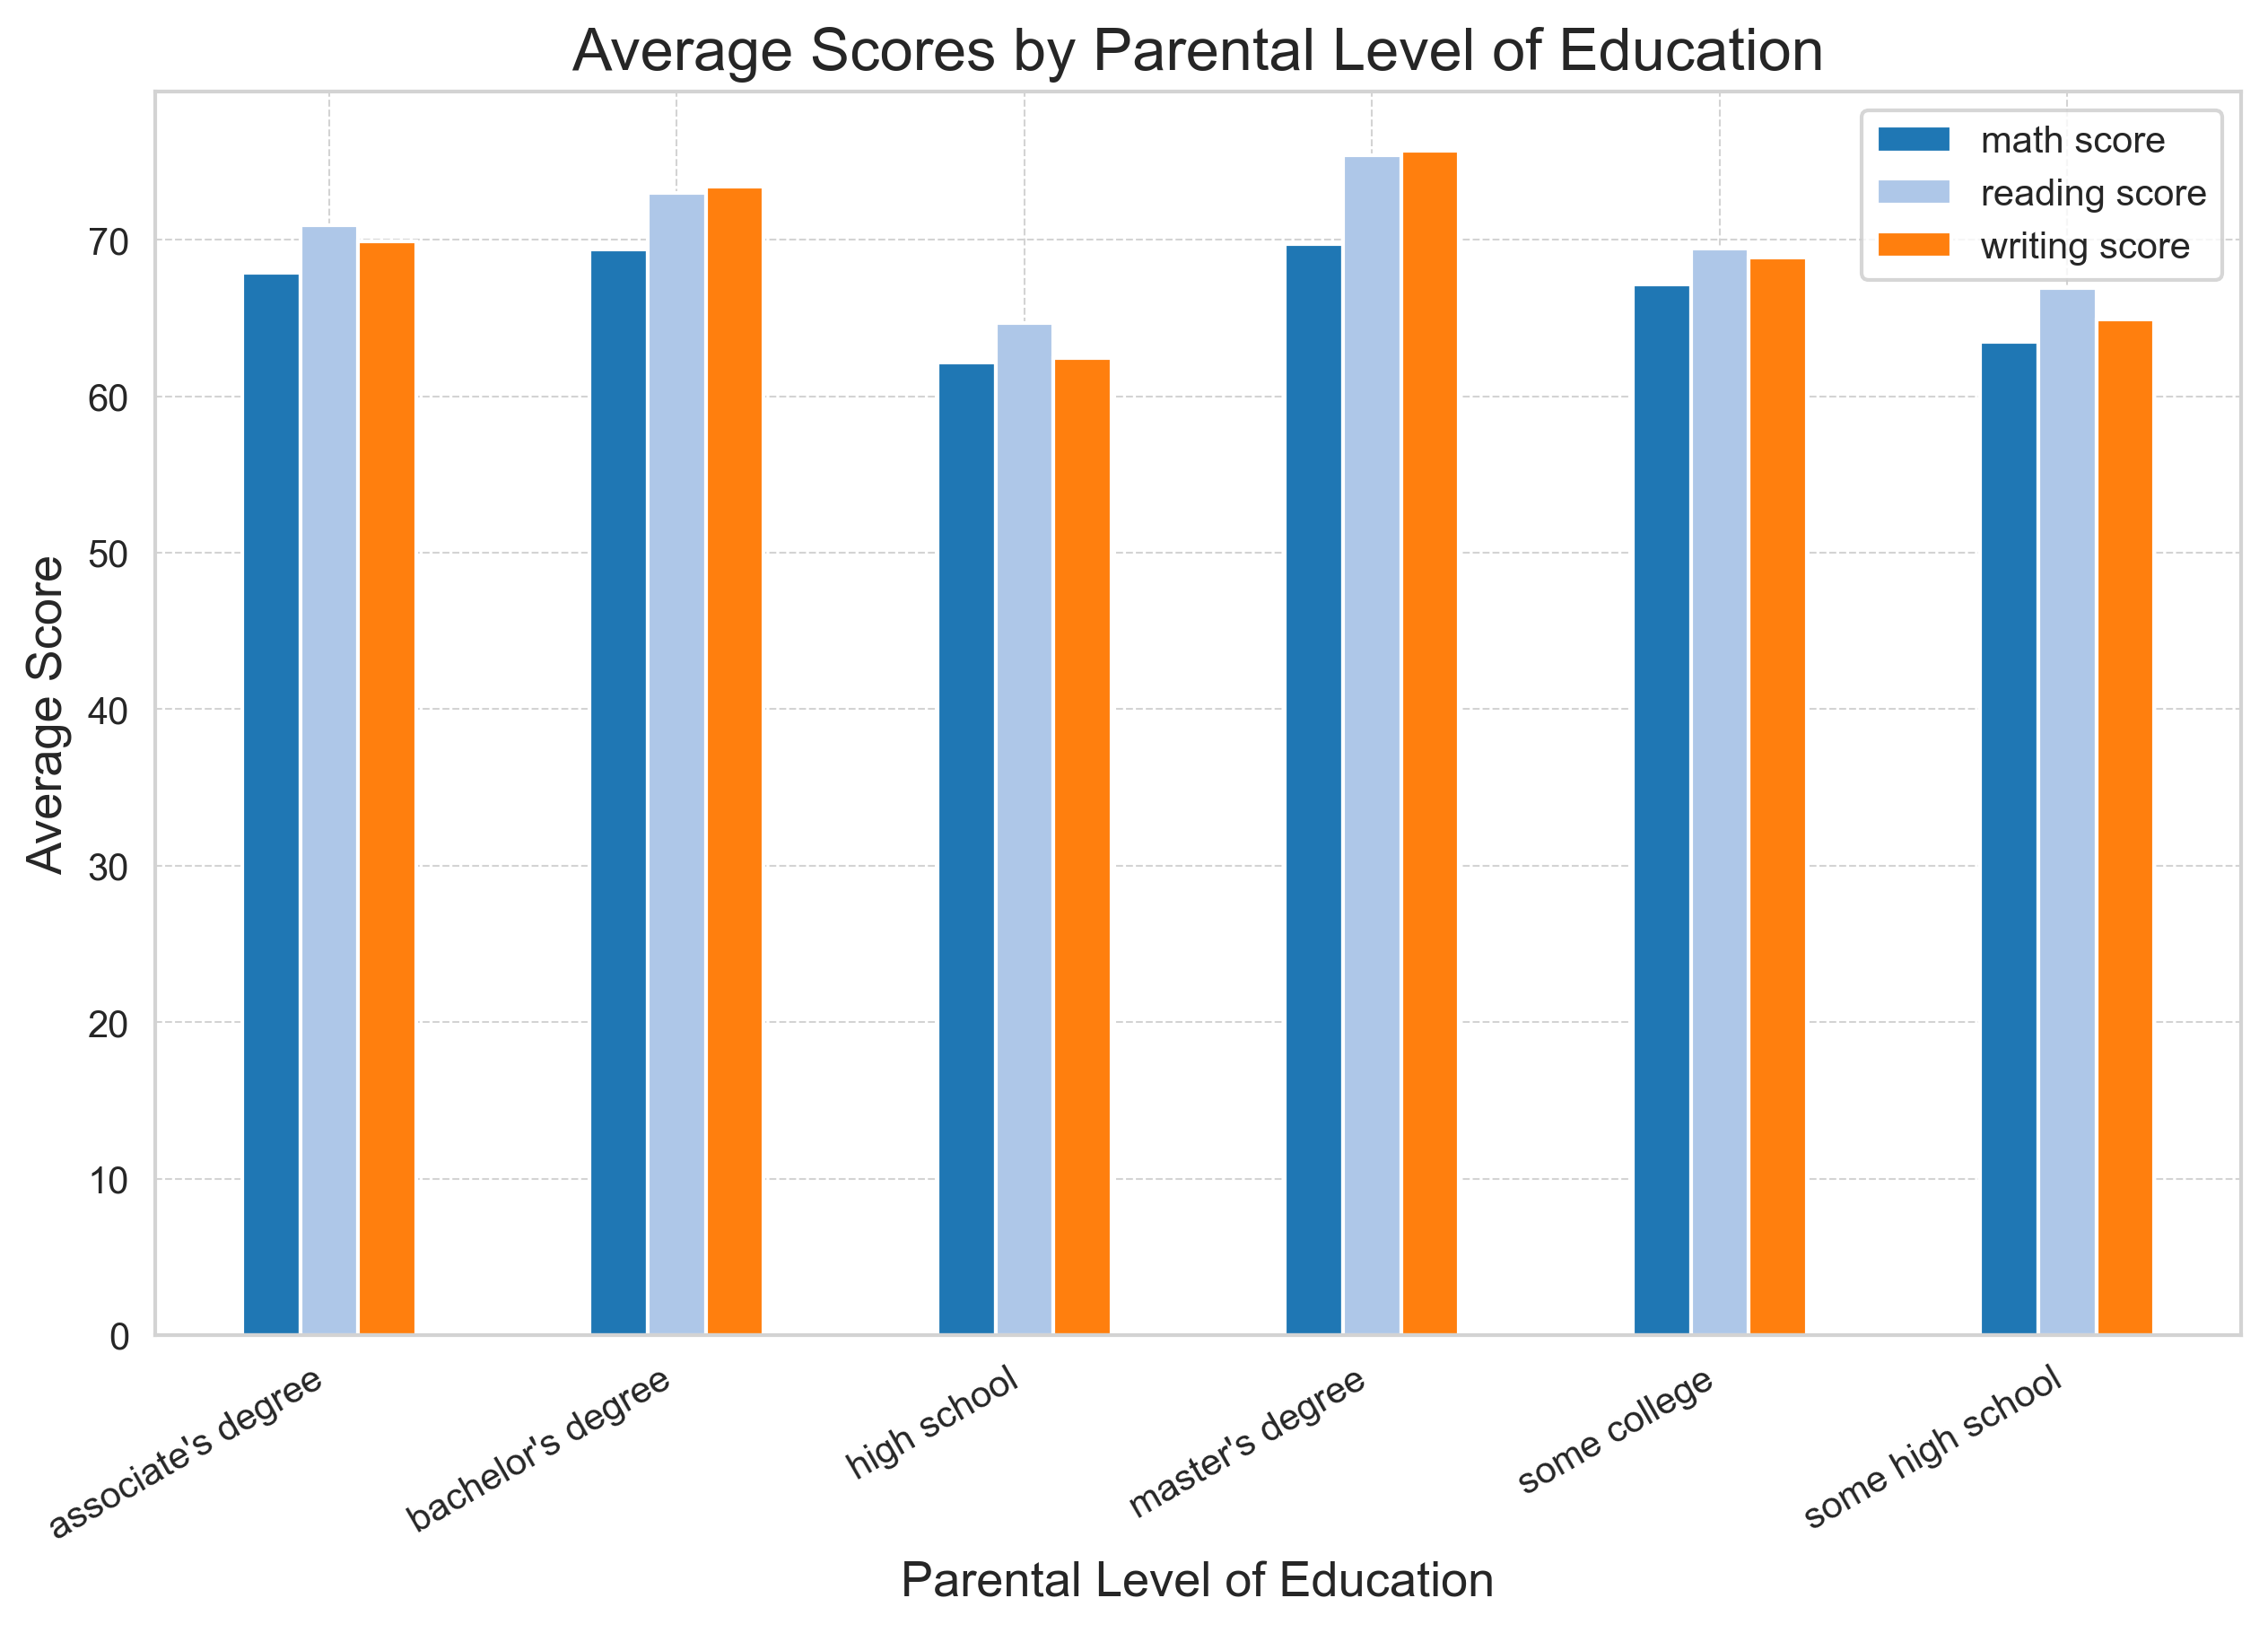
\includegraphics[width=0.8\textwidth]{figures/barchart_avg_scores_by_parent_edu.png}
    \caption{Average Scores by Parental Level of Education}
\end{figure}
\textbf{Key Insight:} Higher parental education levels (bachelor's and master's degrees) are associated with higher student scores across all subjects.

\subsection{Bar Chart: Average Scores by Lunch Type}
\begin{figure}[H]
    \centering
    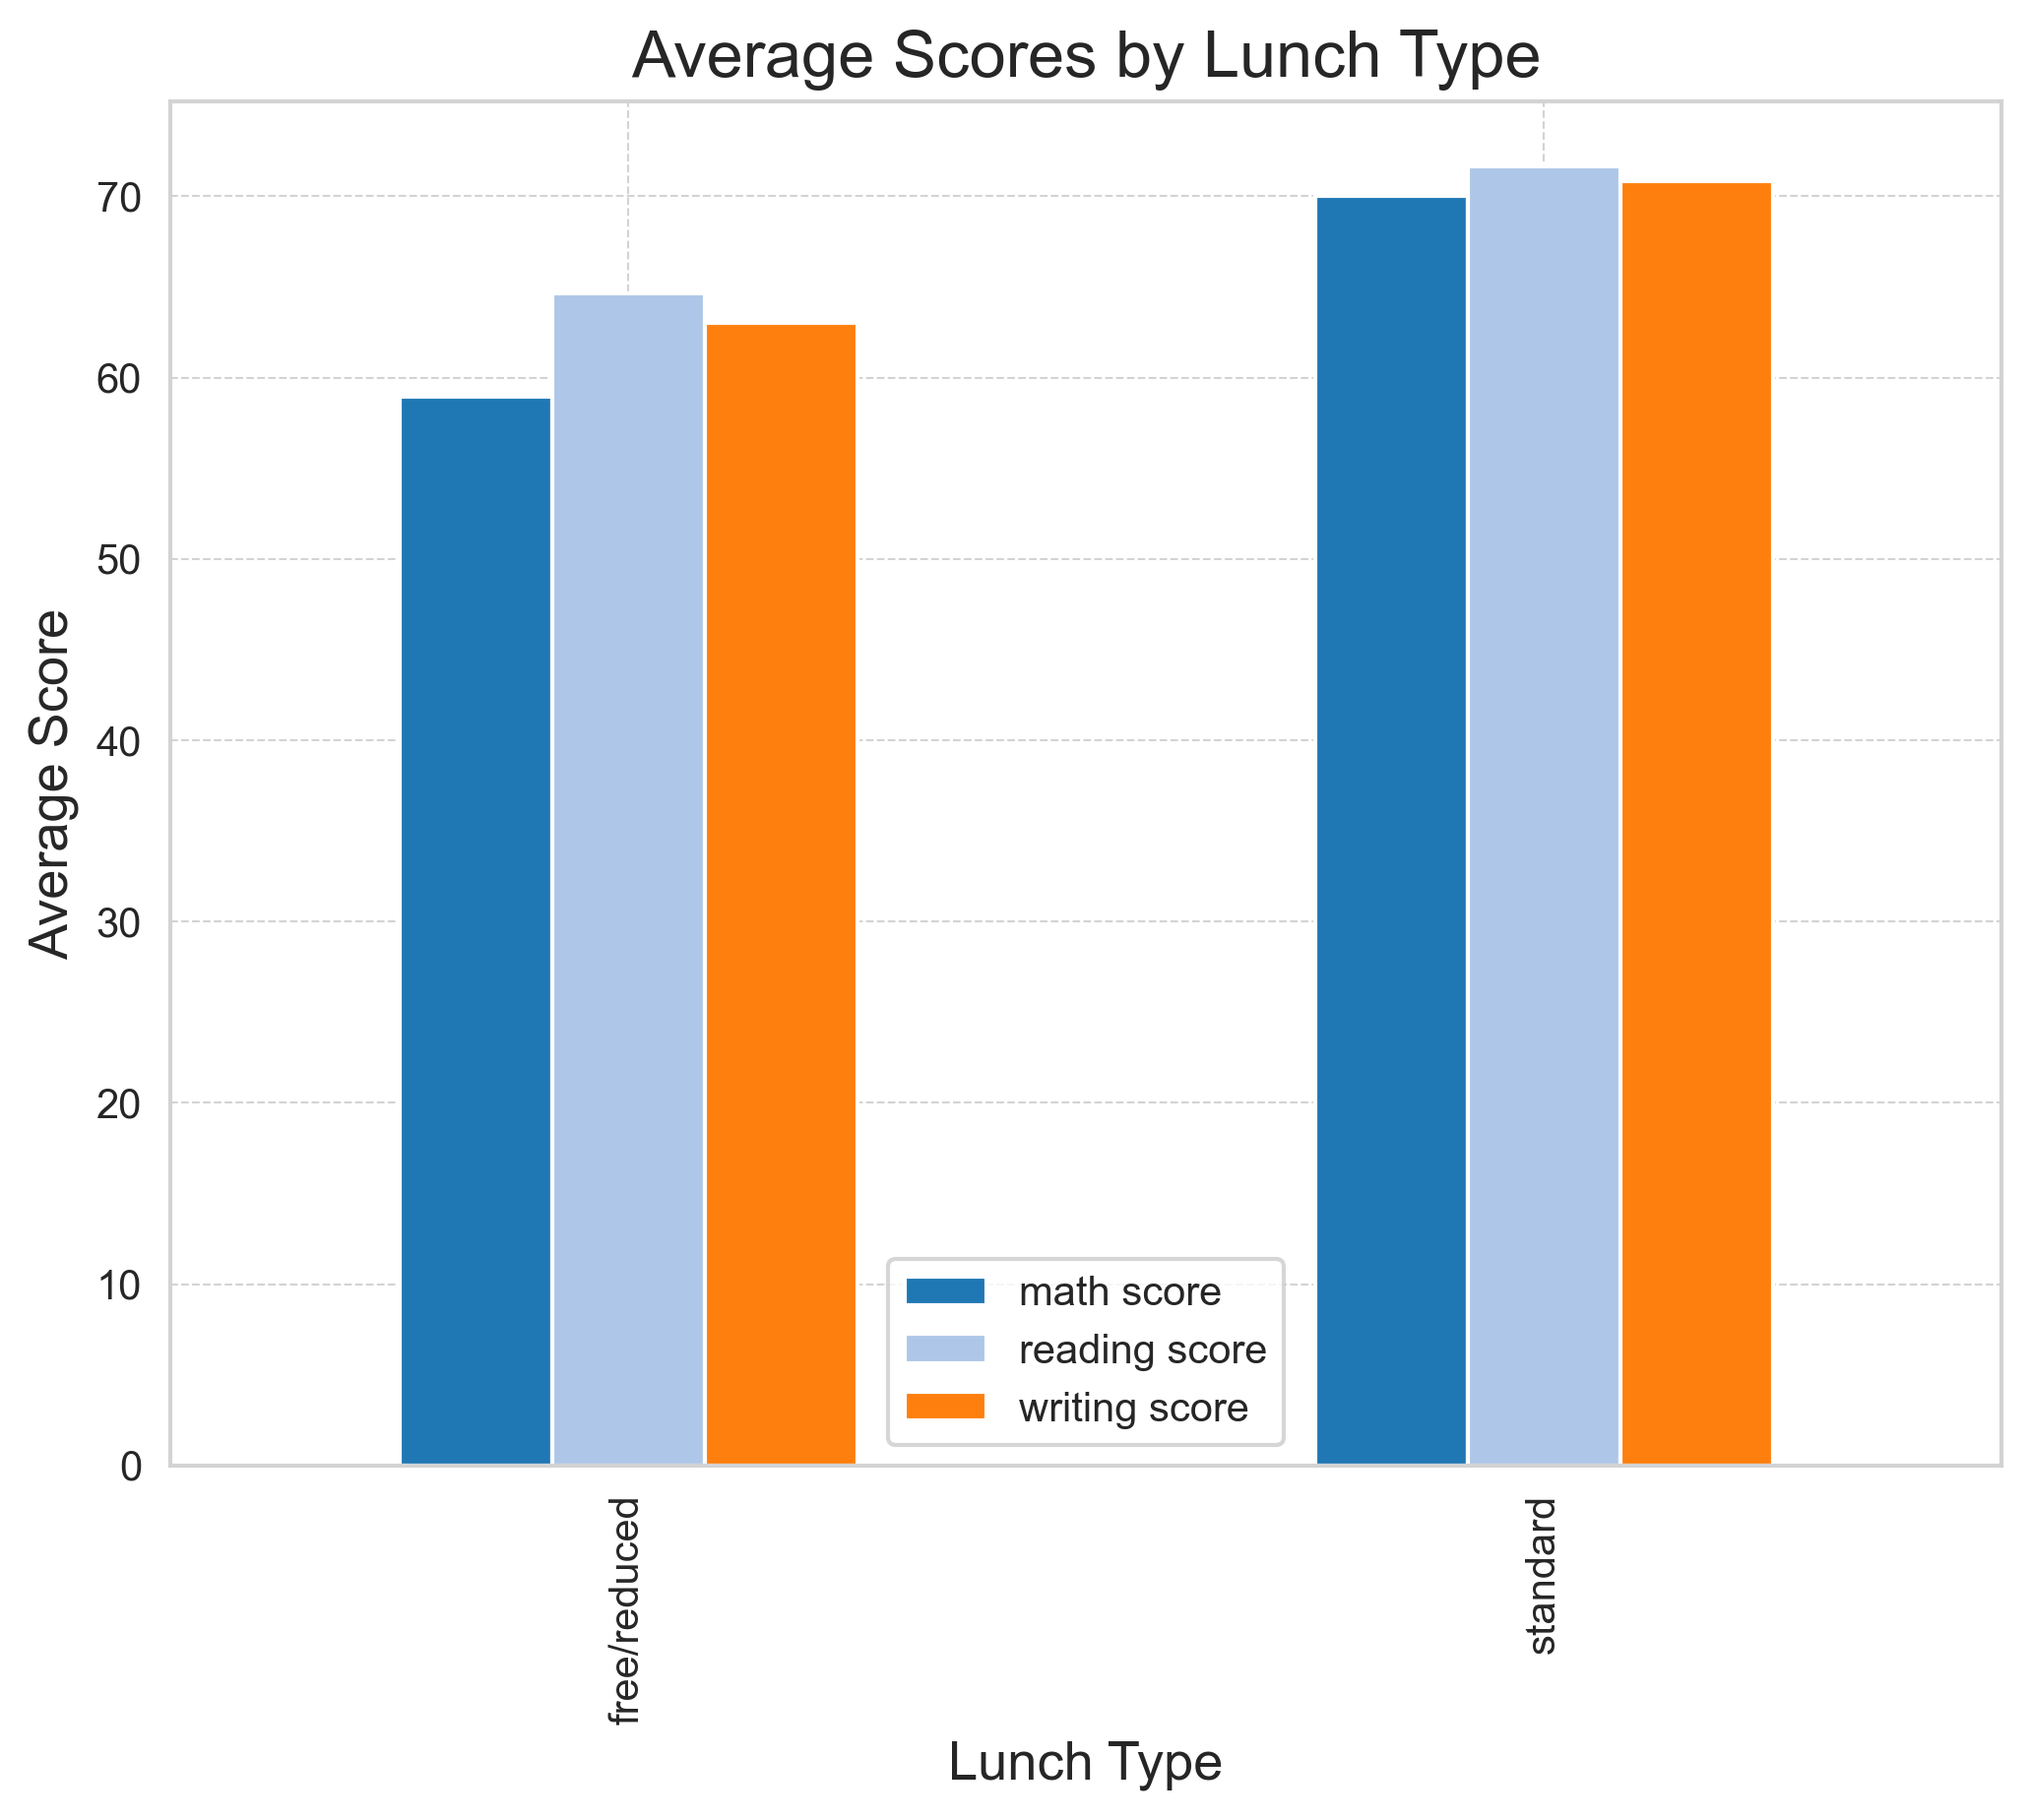
\includegraphics[width=0.8\textwidth]{figures/barchart_avg_scores_by_lunch.png}
    \caption{Average Scores by Lunch Type}
\end{figure}
\textbf{Key Insight:} Students with standard lunch consistently outperform those with free/reduced lunch, indicating a performance gap likely related to socioeconomic status.

\subsection{Bar Chart: Average Scores by Race/Ethnicity}
\begin{figure}[H]
    \centering
    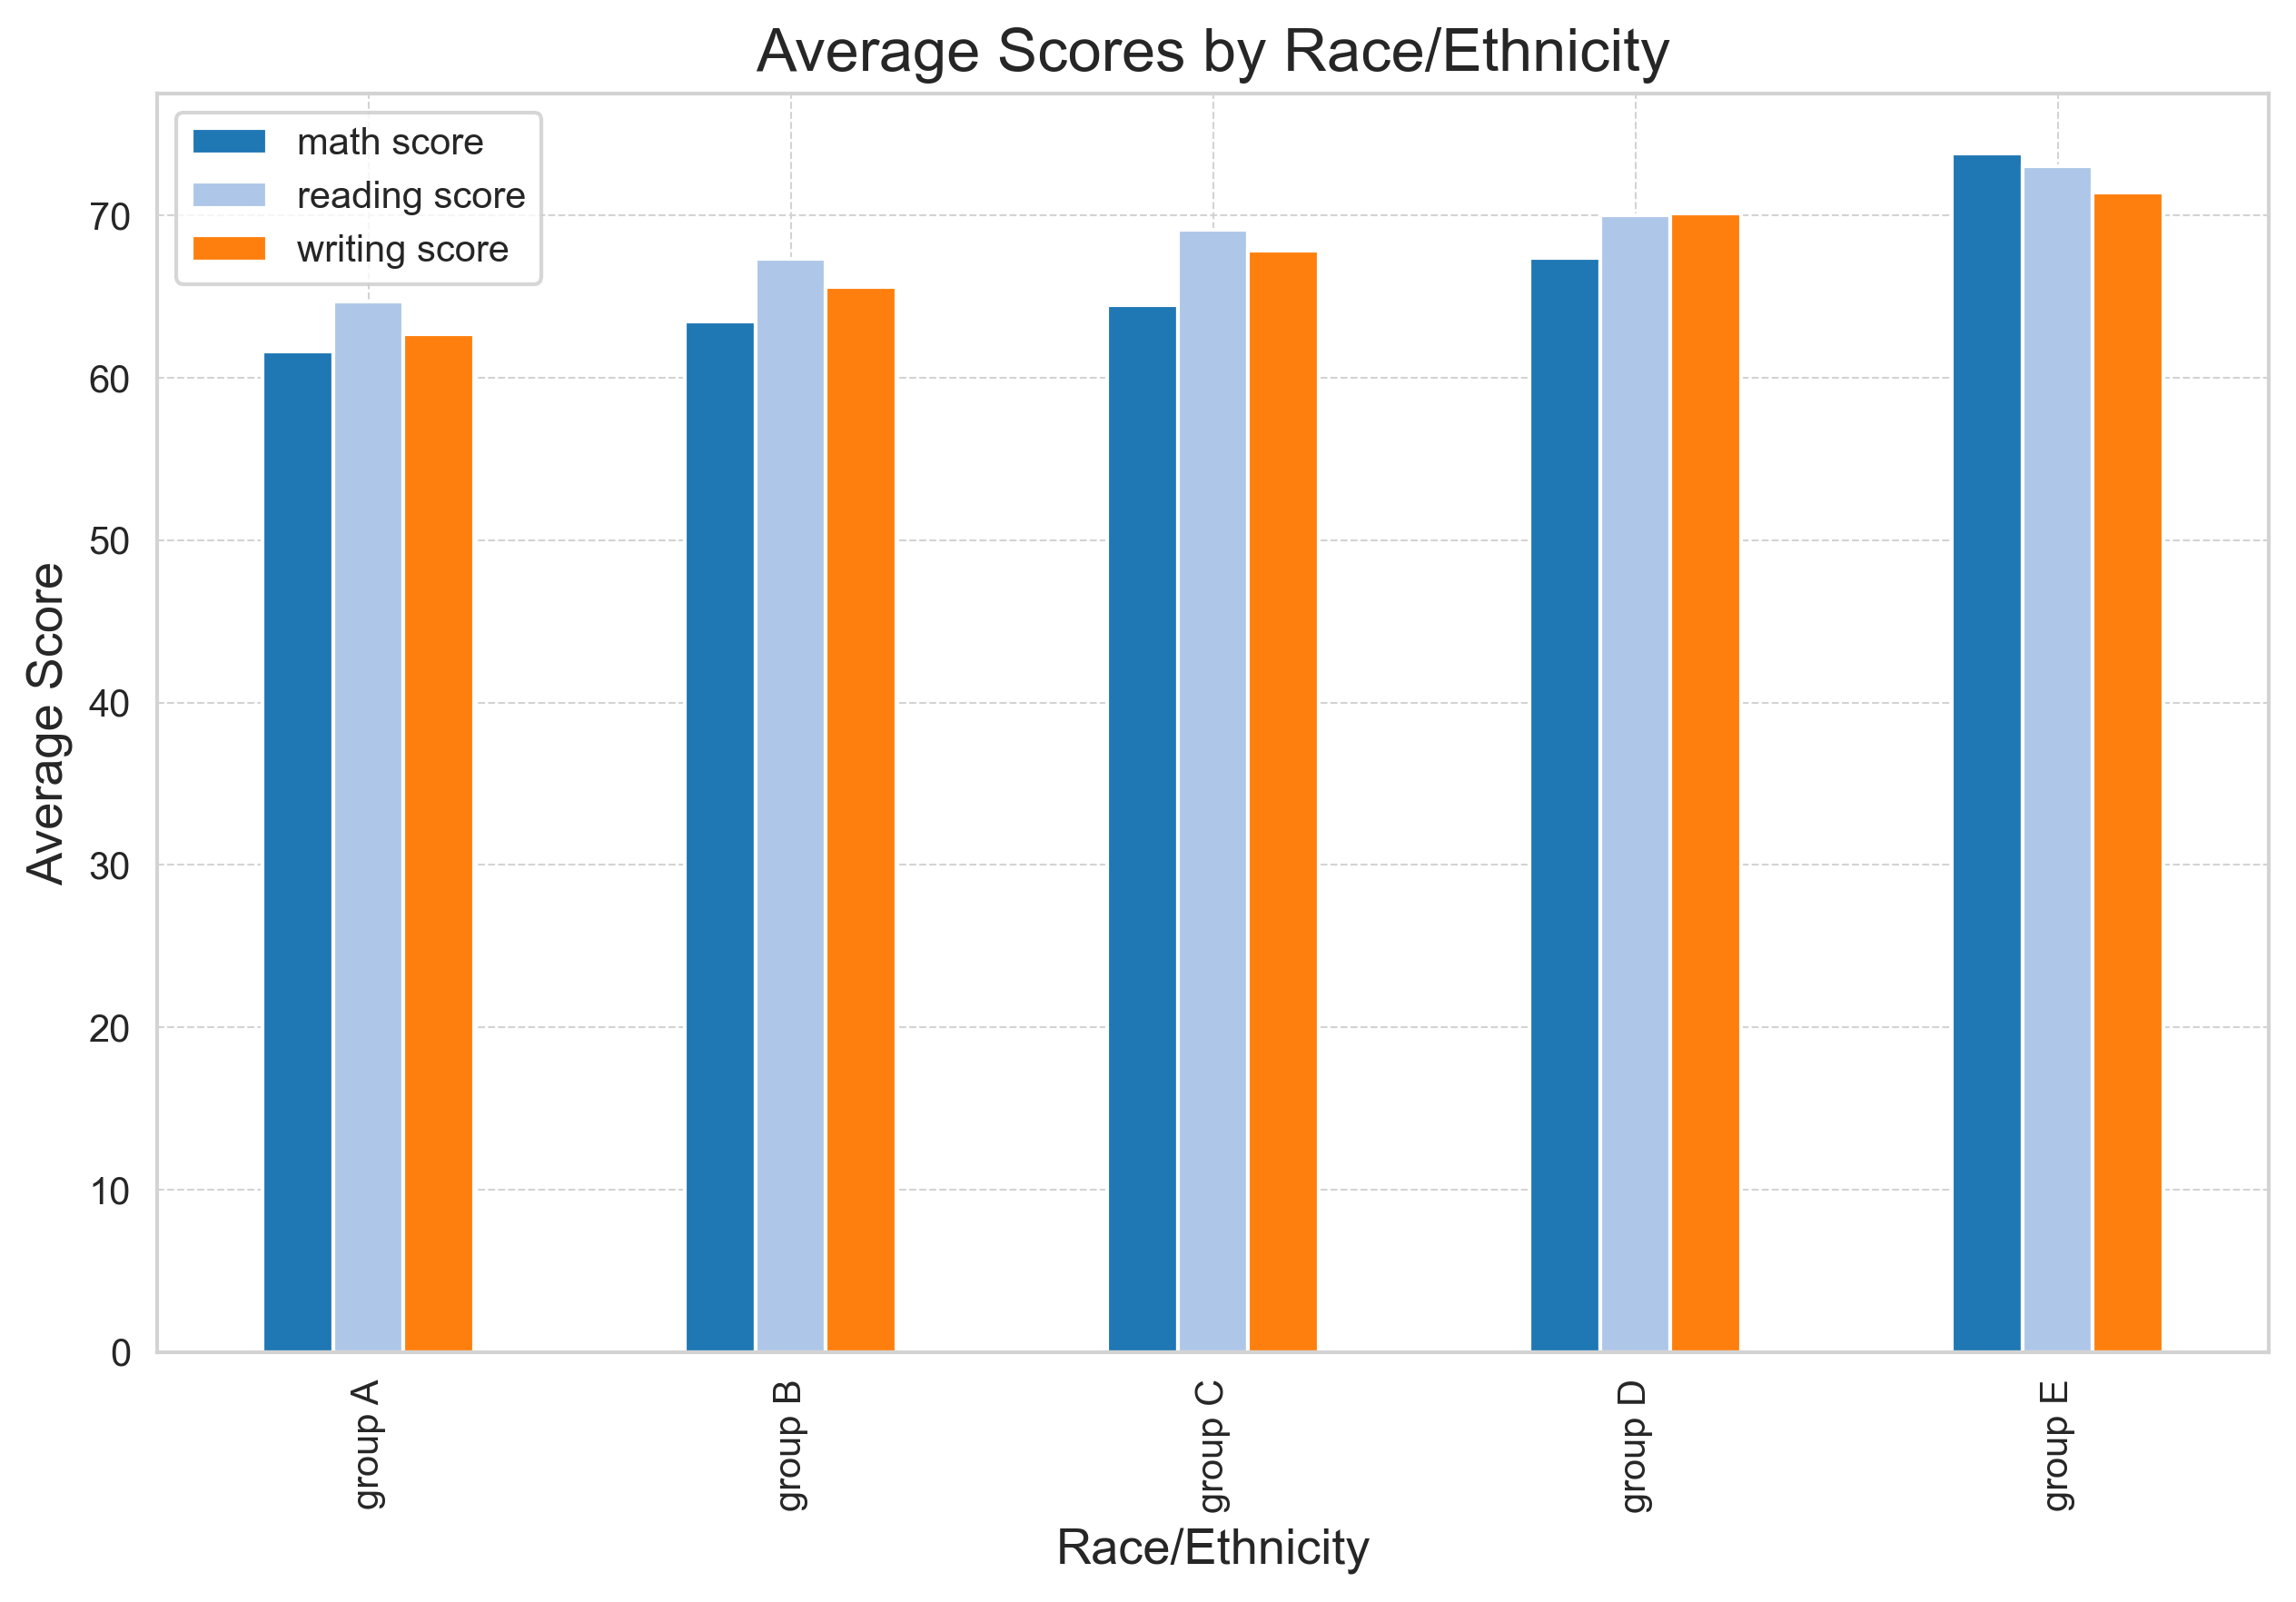
\includegraphics[width=0.8\textwidth]{figures/barchart_avg_scores_by_race.png}
    \caption{Average Scores by Race/Ethnicity}
\end{figure}
\textbf{Key Insight:} Group E students have the highest average scores, while Groups A and B have the lowest. There is a clear upward trend from Group A to Group E.

\subsection{Histogram: Score Distributions}
\begin{figure}[H]
    \centering
    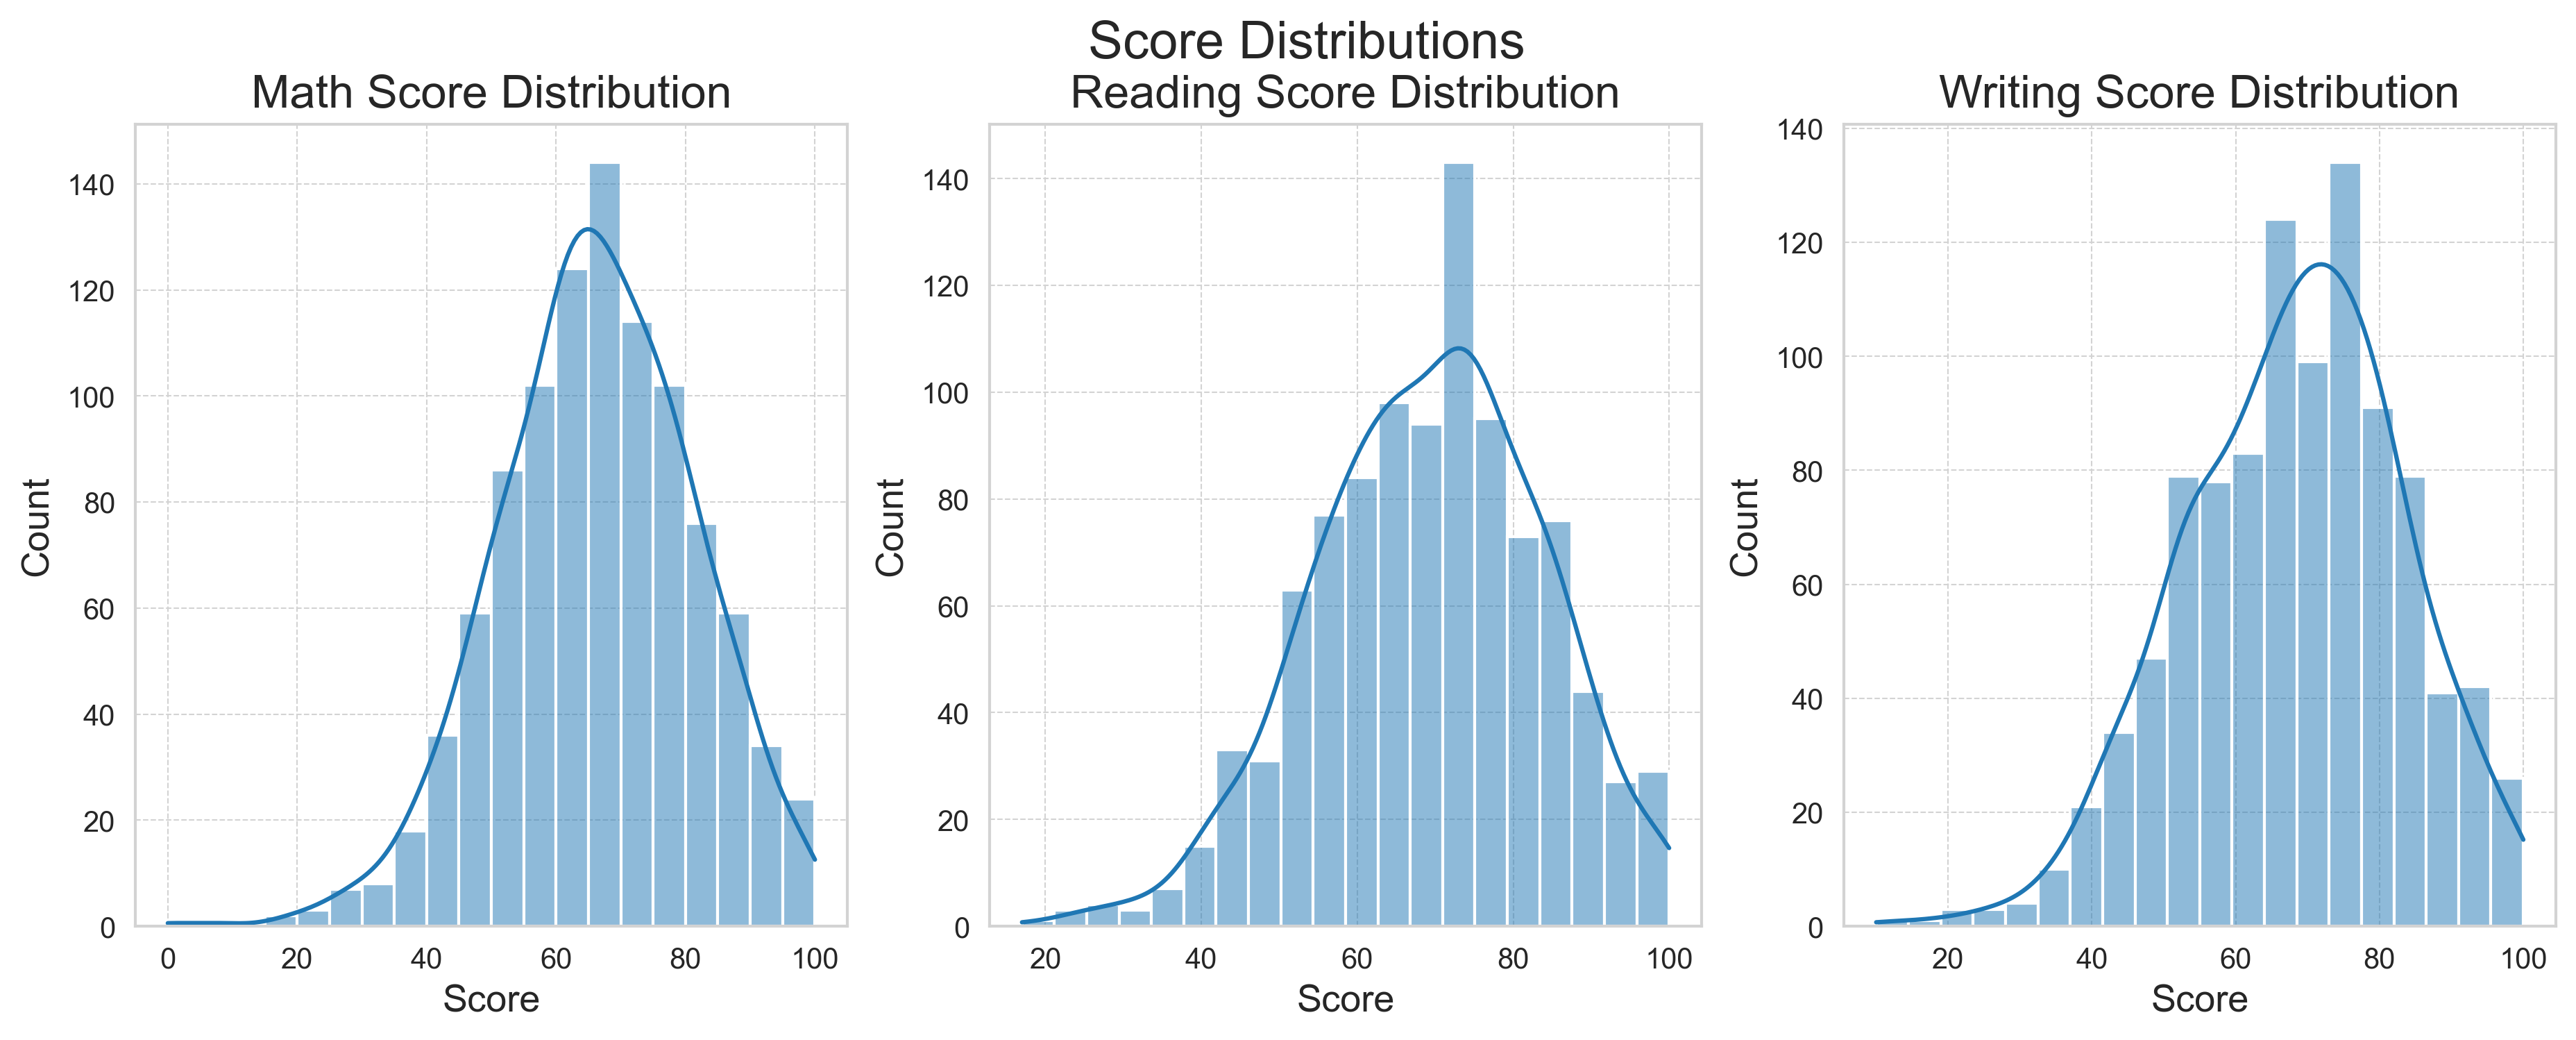
\includegraphics[width=0.8\textwidth]{figures/histograms_scores.png}
    \caption{Distribution of Math, Reading, and Writing Scores}
\end{figure}
\textbf{Key Insight:} Math scores are more widely distributed and skewed lower compared to reading and writing, which are more concentrated at higher values.

\subsection{Correlation Heatmap: Subject Scores}
\begin{figure}[H]
    \centering
    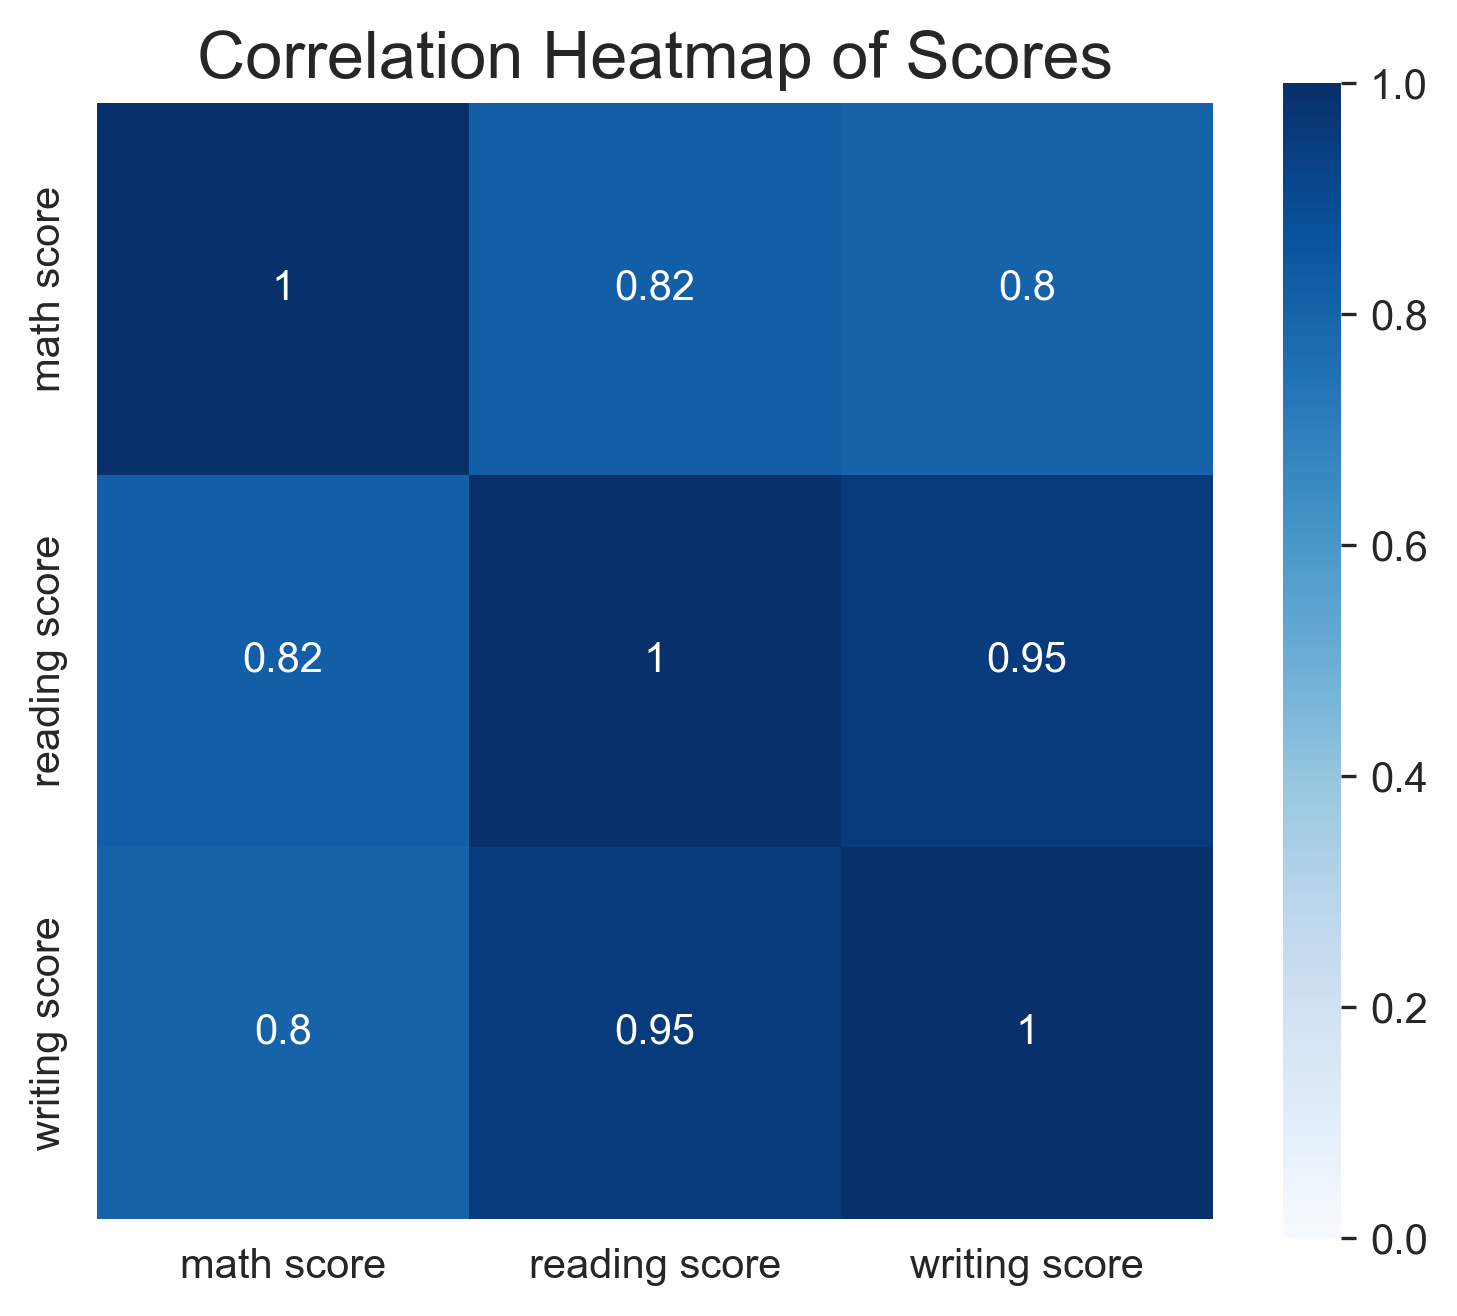
\includegraphics[width=0.6\textwidth]{figures/correlation_heatmap.png}
    \caption{Correlation Heatmap of Math, Reading, and Writing Scores}
\end{figure}
\textbf{Key Insight:} Strong positive correlations exist between all three subjects, especially between reading and writing (0.95).

\subsection{Grouped Bar Chart: Test Preparation Impact by Gender}
\begin{figure}[H]
    \centering
    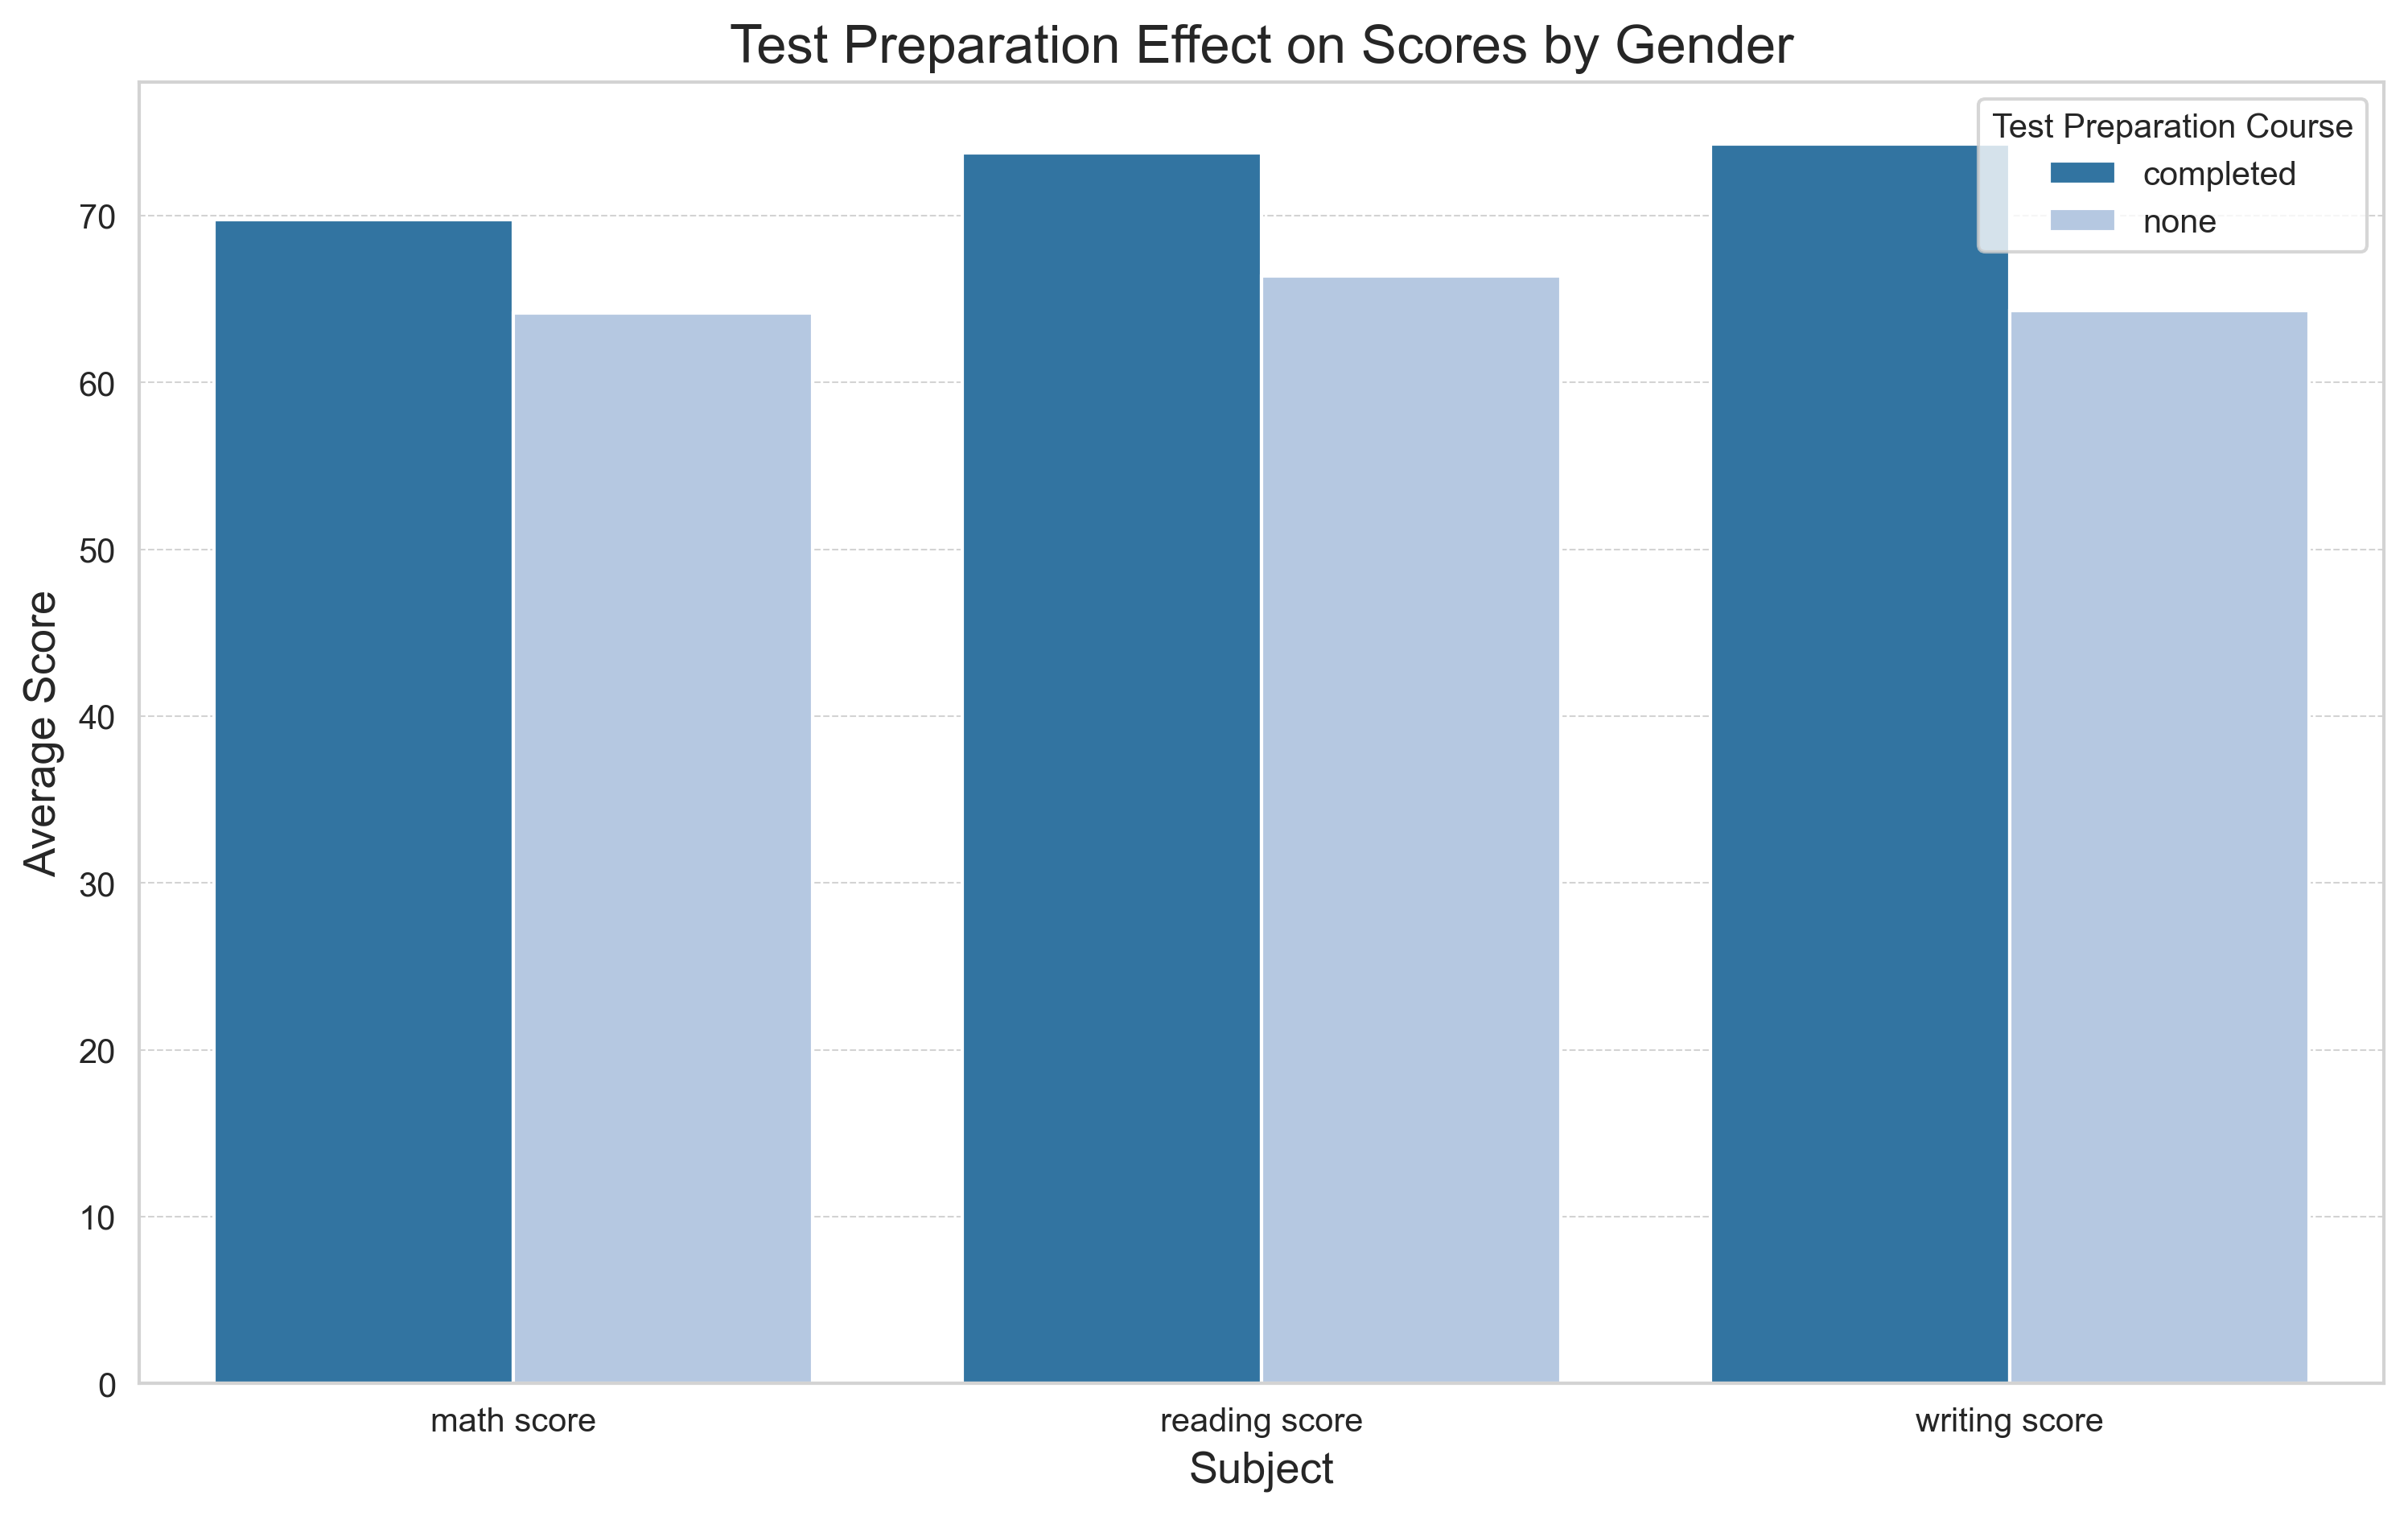
\includegraphics[width=0.8\textwidth]{figures/grouped_barchart_testprep_by_gender.png}
    \caption{Test Preparation Effect on Scores by Gender}
\end{figure}
\textbf{Key Insight:} Test preparation benefits both genders, but the effect is slightly more pronounced for female students in reading and writing.

\section{General Performance Trends and Disparities}
\begin{itemize}
    \item Female students excel in reading and writing; males in math. Socioeconomic and parental education factors strongly influence performance. Test preparation is effective for all groups.
\end{itemize}

\section{Appendix}
\begin{itemize}
    \item Python code and data files available at: \url{https://github.com/dmzinc/visualization-dashboard.git}
\end{itemize}
\end{document} 